
\chapter{Publishing and Querying Geodata }
\label{ch:ch2}

\begin{itemize}
\item steps for publishing geodata--existing tools
\item soA on triple stores 
\item interconnections and 5-stars datasets
\item Datalift for geo data
\item contrib for french publications
\end{itemize}

\section{Existing Tools for Converting Geospatial Data}
\label{sec:toolgeo}

\subsection{Geometry2RDF}

\subsection{TripleGeo}

\subsection{shp2GeoSPARQL}

\subsection{GeoLift}



\section{Geodata Providers and Access}
So far, the Web of data has taken advantage of geocoding technologies for publishing large amounts of data. For example, Geonames provides more than 10 millions records (e.g. $5,240,032$ resources of the form \url{http://sws.geonames.org/10000/}) while LinkedGeoData has more than $60,356,364$ triples. All the above mentioned data are diverse in their structure, the access point (SPARQL endpoint, web service or API), the entities they represent and the vocabularies used for describing them. Table~\ref{tab:srce-data} summarizes for different providers the number of geodata available (resources, triples) and how the data can be accessed.

\begin{table}[!htbp]
\centering{
\begin{tabular}{|ll|r|r|}
\hline
\multicolumn{2}{|c}{\textbf{Provider}} & \multicolumn{1}{|c}{\textbf{\#Geodata}} & \multicolumn{1}{|c|}{\textbf{Data access}}\\
\hline
\multicolumn{2}{|l|}{DBpedia} & 727 232 triples & SPARQL endpoint\\
\multicolumn{2}{|l|}{Geonames} & 5 240 032 (feature). &  API \\
\multicolumn{2}{|l|}{LinkedGeoData} & 60 356 364 triples & SPARQL endpoint, Snorql\\
\multicolumn{2}{|l|}{Foursquare} & n/a & API\\
\multicolumn{2}{|l|}{Freebase} & 8,5MB  & RDF Freebase Service\\
\multicolumn{2}{|l|}{Ordnance Survey(Cities)} & 6 295 triples  & Talis API \\
\multicolumn{2}{|l|}{GeoLinkedData.es} & 101 018 triples  & SPARQL endpoint \\
\multicolumn{2}{|l|}{Google Places} & n/a  & Google API \\
\multicolumn{2}{|l|}{GADM project data} & 682 605 triples & Web Service \\
\multicolumn{2}{|l|}{NUTS project data} & 316 238 triples & Web Service \\
\multicolumn{2}{|l|}{IGN experimental} & 629 716 triples & SPARQL endpoint \\
\hline
\end{tabular}
\caption{Geodata by provider and their different access type}
\label{tab:srce-data}
}
\end{table}



\section{Scenario: 7$^{th}$ Arrondissement of Paris}                      \label{sec:scenario}
\todo{Update the scenario with the current version of DBpedia 2014, DBpedia-FR}

The 7$^{th}$ arrondissement of Paris is one of the 20 arrondissements (administrative districts) of the capital city of France. It includes some of Paris's major tourist attractions such as the Eiffel Tower, some world famous museums (e.g: \textit{mus\'{e}e d'Orsay}) and contains a number of French national institutions, including numerous government ministries\footnote{\url{http://en.wikipedia.org/wiki/7th_arrondissement_of_Paris}}. We use it throughout this paper to highlight the diversity of representations one can use for this geographical entity. We assume that this district should be modeled as a POLYGON composed of a number of POINTs needed to ``interpolate'' its effective boundaries. We assume the use of the WGS84\footnote{\url{http://en.wikipedia.org/wiki/World_Geodetic_System}} geodetic system.

\subsection{DBpedia Modeling}
We provide below an excerpt of the DBpedia description for this resource.
{\scriptsize
\begin{verbatim}
  dbpedia:7th_arrondissement_of_Paris a gml:_Feature ;
    a <http://dbpedia.org/class/yago/1900SummerOlympicVenuEs>
    rdfs:label "7. arrondissementti (Pariisi)"@fi; (14 different languages)
    dbpprop:commune "Paris" ;
    dbpprop:departement  dbpedia:Paris ;
    dbpprop:region dbpedia:Ile-de-France_(region) ;
    grs:point "48.85916666666667 2.312777777777778" ;
    geo:geometry "POINT(2.31278 48.8592)" ;
    geo:lat "48.859165"^^xsd:float;
    geo:long "2.312778"^^xsd:float.
\end{verbatim}
}
First, we observe that the type \texttt{gml:\_Feature} and the property \texttt{grs:point} are not resolvable since there are no OWL ontologies that provide a description of them. Second, the property \texttt{geo:geometry} used by DBpedia is not defined in the WGS84 vocabulary. For the geometry, the 7th arrondissement is a simple POINT defined by a latitude and a longitude.

\subsection{Geonames Modeling}
In Geonames, the 7th arrondissement is considered as a 3$^{rd}$ order administrative division, represented by a POINT for the geometry model. The RDF description of this resource gives other information such as the alternate name in French, the country code and the number of inhabitants.
{\scriptsize
\begin{verbatim}
  gnr:6618613 a gn:Feature ;
    gn:name "Paris 07";
    gn:alternateName "7ème arrondissement";
    gn:featureClass gn:A [
      a skos:ConceptScheme ;
      rdfs:comment "country, state, region ..."@en .
    ] ;
    gn:featureCode gn:A.ADM4 [
      a skos:Concept ;
      rdfs:comment "a subdivision of a third-order administrative division"@en .
    ];
    gn:countryCode "FR";
    gn:population "57410";
    geo:lat "48.8565";
    geo:long "2.321".
\end{verbatim}
}

\subsection{LinkedGeoData Modeling}
In LinkedGeoData, the district is a \texttt{lgdo:Suburb rdfs:subClassOf ldgo:Place}. Its geometry is still modeled as a POINT and not as a complex geometry of type POLYGON as we could have expected for this type of spatial object.
{\scriptsize
\begin{verbatim}
  lgd:node248177663 a lgdo:Suburb ;
    rdfs:label "7th Arrondissement"@en , "7e Arrondissement" ;
    lgdo:contributor lgd:user13442 ;
    lgdo:ref%3AINSEE 75107 ;
    lgdp:alt_name "VIIe Arrondissement" ;
    georss:point "48.8570281 2.3201953" ;
    geo:lat 48.8570281 ;
    geo:long 2.3201953 .
\end{verbatim}
}

\subsection{Linked Geospatial Data for Greece}
\todo{add a representation of data here}\\

Linked Geospatial Data for Greece - http://www.linkedopendata.gr/ - Linked geospatial data about the Greek Administrative Geography, CORINE Land Use/Land Cover for Greece and the Coastline of Greece.

\subsection{Discussion}
These samples from DBpedia, Geonames and LinkedGeoData give an overview of the different views of the same reality, in this case the district of the 7$^{th}$ Arrondissement in Paris. Regarding the ``symbolic representation'', two datasets opted for ``Feature'' (DBpedia and Geonames) while LGD classifies it as a ``Suburb'' or ``Place''. They all represent the shape of the district as a POINT which is not very efficient if we consider a query such as \emph{show all monuments located within the 7th arrondissement of international importance}. To address this type of query and more complicated ones, there is a need for more advanced modeling as we describe in the next section.

\section{Benchmarking Triple Stores}
\label{sec:benchmarking}

\begin{itemize}
\item \textbf{Serialization and Triple stores:} We also advocate the use of properties that can provide compatibility with other formats (GML, KML, etc.). This choice can be triple store independent, as there could be ways to use content-negotiation to reach the same result. In Table \ref{tab:triplestore}, \texttt{Open Sahara}\footnote{\url{http://www.opensahara.com}}, \texttt{Parliament }\footnote{\url{http://geosparql.bbn.com}},  \texttt{Virtuoso}\footnote{\url{http://www.openlinksw.com}} are WKT/GML-compliant with respectively $23$ and $13$ functions dealing with geodata.
\item The choice of the triple store (e.g.,Virtuoso\footnote{Here we used Virtuoso Open Edition, V6.xx} vs Open Sahara) is not really an issue, as the IndexingSail\footnote{\url{https://dev.opensahara.com/projects/useekm/wiki/IndexingSail}} service could also be wrapped on-top of Virtuoso to support full OpenGIS Simple Features functions\footnote{\url{http://www.opengeospatial.org/standards/sfs}}.
\end{itemize}

\todo{update the table with strabon and changes in virtuoso 7.} \\

\subsection{Strabon}
\todo{read again the paper}
Strabon - http://www.strabon.di.uoa.gr - Strabon is a semantic spatio-temporal RDF store. You can use it to store linked geospatial data that changes over time and pose queries using two popular extensions of SPARQL. Strabon is a full implementation of stSPARQL and the GeoSPARQL Core, Geometry extension and Geometry topology extension components. It also offers spatial and temporal selections, spatial and temporal joins, a rich set of spatial functions similar to those offered by geospatial relational database systems and support for multiple Coordinate Reference Systems.

\begin{table}[!htbp]
 \begin{tabularx}{\textwidth}{|X|X|X|X|X|l|}
 \hline
 \textbf{Triple store} & WKT-compliance & GML-compliance & Geometry supported  & Geospatial Functions & GeoVocab \\ \hline
 Virtuoso & Yes & Yes & Point & 13 functions & W3C Geo + Typed Literal  \\ \hline
 Allegro-Graph & \-- & -- & Point & 3 functions & ``strip'' mapping data \\ \hline
 OWLIM-SE & -- & -- & Point & 4 functions & W3C Geo\\ \hline
 Open Sahara & \ Yes & Yes & Point, Line, Polygons & 23 functions  & Typed Literal \\ \hline
 Parliament & \ Yes & Yes & Point, Line, Polygons & 23 functions  &  GeoSPARQL vocabulary\\ \hline
 \end{tabularx}
\caption{Triple stores survey with respect to geometry types supported and geospatial functions implemented.}
\label{tab:triplestore}
\end{table}

\subsection{Benchmarks}
Geographica - http://geographica.di.uoa.gr - A benchmark which uses both real-world and synthetic data to test the offered functionality and the performance of some prominent geospatial RDF stores.

\section{Tools for managing Linked (Geo)Data Publishing Workflow}
\label{sec:toolLD}

\subsection{GeoKnow}
\label{sec:geoknow}

\subsubsection{LIMES}
\todo{rewrite this section and add references of Axel Papers}
LIMES is an abbreviation of the LInk discovery framework for MEtric Spaces, a tool for interlinking resources on the Web of Data\footnote{\url{At http://aksw.org/Projects/LIMES.html}}. It implements time-efficient approaches for large-scale link discovery based on the characteristics of metric spaces. It is easily configurable via a web interface. It can also be downloaded as standalone tool for carrying out link discovery locally.
LIMES implements novel time-efficient approaches for link discovery in metric spaces. Its approaches different approximation techniques to compute estimates of the similarity between instances. These estimates are then used to filter out a large amount of those instance pairs that do not suffice the mapping conditions. By these means, LIMES can reduce the number of comparisons needed during the mapping process by several orders of magnitude. The approaches implemented in LIMES include the original LIMES algorithm for edit distances, REEDED for weighted edit distances, HR3, HYPPO, and ORCHID. Moreover, LIMES implements supervised and unsupervised machine-learning algorithms for finding accurate link specifications. The algorithms implemented here include the supervised, active and unsupervised versions of EAGLE, COALA and EUCLID.

\subsection{Datalift Platform}
\label{sec:datalift}
Datalift is an open source platform [ref-datalift] helping to lift raw data sources or legacy data to semantic interlinked data sources.
The ambition of DataLift is to act as a catalyst for the emergence of the Web of Data by providing a complete path from raw data to fully interlinked, identified, and qualified linked datasets. The Datalift platform supports the following stages in lifting the data:
\begin{enumerate}
\item Selection of ontologies for publishing data;
\item Conversion of data to the appropriate format (e.g., from CSV to RDF);
\item Interlinking of data with other data sources;
\item Publication of linked data ;
\item Access control and license management
\end{enumerate}



\subsubsection{Functionalities of the Datalift platform}

The architecture of Datalift is modular. Several levels of abstraction allow decoupling between the different stages from raw data to semantic data. The dataset selection allows us to identify the data to be published and migrate them to a first RDF version. The ontologies selection step asks the user to input a set of vocabularies', terms that will be used to describe the lifted data. Once the terms are selected, they can be mapped to the raw RDF and then converted to properly formatted RDF. The data is then published on the DataLift SPARQL endpoint. Finally, the process aims at providing links from the newly published data to other datasets already published as Linked Data on the Web. Figure \ref{fig:liftprocess} below shows the workflow of converting raw data into ``structured'' RDF data.


\begin{enumerate}

\item{Dataset Selection}
The first step of the data lifting process is to identify and access the datasets to be processed. A dataset is either a file or the result of a query to retrieve data from a datastore. The kinds of files currently considered are CSV, RDF, XML, GML and Shape files. Queries are SQL queries sent to an RDBMS or SPARQL queries on a triple store.
\item{Ontologies Selection:}
The publisher of a dataset should be able to select the vocabularies that are the most suitable to describe the data, and the least possible terms should be created specifically for a dataset publication task. The Linked Open Vocabularies[1] (LOV) developed in Datalift provides easy access methods to this ecosystem of vocabularies, and in particular by making explicit the ways they link to each other and providing metrics on how they are used in the linked data cloud. LOV is integrated as module in the DataLift platform to assist the ontology selection.
\item{Data Conversion:}
Once URIs are created and a set of vocabulary terms able to represent the data is selected, it is time to convert the source dataset into a more precise RDF representation. Many tools exist to convert various structured data sources to RDF. The major source of structured data on the Web comes from spreadsheets, relational databases and XML files. We propose a two steps approach. First, a conversion from the source format to raw RDF is performed. Second, a conversion of the raw RDF into ``well-formed'' RDF using selected vocabularies is performed using SPARQL Construct queries. Most tools provide spreadsheet conversion to CSV, and CSV to RDF is straightforward, each line becoming a resource, and columns becoming RDF properties. The W3C RDB2RDF WG\footnote{\url{http://www.w3.org/2001/sw/rdb2rdf/}} proposes the Direct Mapping to automatically generate RDF from the tables but without using any vocabulary, and R2RML\footnote{\url{http://www.w3.org/TR/r2rml/}}  to assign vocabulary terms to the database schema. In the case of XML, a generic XSLT transformation is performed to produce RDF from a wide range of XML documents. The DataLift platform provides a graphical interface to help mapping the data to selected vocabulary terms.
\item{\textbf{Data Protection:}}
This module is linked to Apache Shiro for obtaining the information, i.e., username and password, about the user who is accessing the platform. The module\footnote{\url{http://wimmics.inria.fr/projects/shi3ld/}} checks which data is targeted by the user's query and then verifies whether the user can access the requested data. This verification leads to three kinds of possible answers, depending on the access privileges of the user: some of the requested data is returned, all the requested data is returned, or no data is returned. This means that the user's query is filtered in such a way that she is allowed to access only the data she is granted access to. The access policies are expressed using RDF and SPARQL 1.1[ref-sparql11] Semantic Web languages thus provide a completely standard way of expressing and enforcing access control rules.
\item{\textbf{Data Interlinking:}}
The interlinking step provides means to link datasets published through the Datalift platform with other datasets available on the Web of Data. Technically, the module helps to find equivalence links in the form of ``owl:sameAs'' relations. An analysis of the vocabulary terms used by the published data set and a potential data set to be interlinked is performed. When the vocabulary terms are different, the module checks if alignments between the terms used by the two data sets are available.Here the alignment server provided with the Alignment API\footnote{\url{http://alignapi.gforge.inria.fr/}} is used for that purpose. The correspondences are translated into SPARQL graph patterns and transformation functions are combined into a SILK script.
\item{\textbf{Data Publication:}}
This module aims at publishing the data obtained from the previous steps to a triple store, either public or private. The providers can restrict which graphs can be accessible, they could decide whether to provide just a ``Linked Data'' or a ``Linked Open Data''. Datalift comes by default with Sesame , but provides API for connecting to Allegrograph, OWLIM, and Virtuoso triple stores as well.
\end{enumerate}


\begin{figure}[!htp]
\centering{
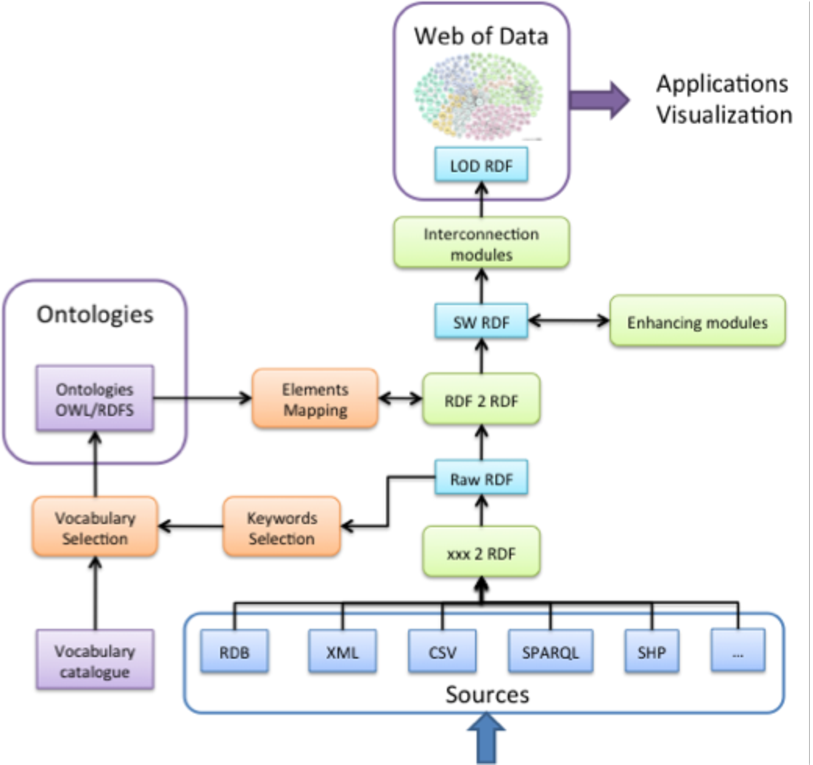
\includegraphics[scale=0.9]{img/liftProcessDatalift.pdf}
\caption{Lifting process of raw data source into RDF using Datalift Platform}
\label{fig:liftprocess}
}
\end{figure}

\paragraph{Installation:}
Please find the documentation for installing Datalift at \url{http://datalift.org/wiki/index.php/Platform_installation_(english)}. The latest version of the platform is available at http://datalift.org/en/node/24, which is still a work in progress until the mature and stable version is released by the end of March. 

\paragraph{Usage:}
The data lifting has several distinct steps. DataLift makes it possible to replay each step in producing different results for each step. To facilitate access to all the different treatments and their results, they are grouped as one project. The project gathers together the various sources used and the results of all treatments done.
Each module has its own way to be used within the lifting process in DataLift. For more details, the readers are encouraged to read this resource at \url{http://datalift.org/wiki/index.php/How_to_use_the_Datalift_platform_to_publish_a_dataset_on_the_Web#The_lifting_project. 
}


\subsection{Comparison Geoknow vs Datalift}

\todo{add here the comparison}

\section{Publishing French Administrative Units (GeoFla)} \label{sec:geofla}
As a dataset dedicated to administrative units, GEOFLA\circledR is very likely to be reused by other datasets, either by reusing directly its URIs for georeferencing needs, or by reusing its description of administrative units - labels, properties and geometries - for interlinking purposes. 

\subsection{Data conversion}
\label{sec:dconversion}
Geofla  is delivered as a set of 4 shapefiles  that describe the boundaries and properties of administrative units of mainland France (for CRS reasons, overseas territories are delivered within different shapefiles) : communes, cantons, arrondissements and departements. For the sake of our application, we have generated another shapefile describing regions by aggregating the geometries of the instances of departments based on their region's foreign key value. This  dataset is updated every year.  Publishing this data in RDF with unique identifiers on the Web will ease the interlinking with some existing datasets describing French boundaries in the wild. We follow a two steps conversion: we use the SHP2RDF module of Datalift to obtain a raw RDF from shapefiles, and the RDF2RDF module of Datalift  using a set of SPARQL construct queries\footnote{ \url{https://github.com/gatemezing/ign-iswc2014/tree/master/rdf2rdf}} for getting a refined RDF datasets using suitable vocabularies.

\subsection{URI design policy} \label{sec:urigeofla}

One of the requirements to publish data is to have unique ids and stable URIs\footnote{\url{http://www.w3.org/TR/ld-bp/}} . Since our legacy databases have unique IDs to refer to the objects, we had to make sure they were unique at Web level. Thus, the base scheme for vocabularies URIs is: \url{http://data.ign.fr/def/}. Besides, the base schema for identifying a real world resource uses \url{http://{BASE}/id/}. For example, IGN main buildings  are located in the commune with the URI \url{rgeofla:commune/94067}, corresponding to Saint-Mand\'{e}, and \url{rgeofla:departement/94} corresponds to the department ``Val de Marne'' to which the commune belongs.

%We had to make choices based on the set of best practices related to URI design\footnote{\url{http://www.w3.org/TR/ld-bp/#HTTP-URIS}} which should guarantee stable and human readable identifiers.


\subsection{Interlinking with existing GeoData} \label{sec:mapping}
We interlinked our datasets with NUTS, DBpedia FR\footnote{\url{http://fr.dbpedia.org/}} and GADM datasets. SILK \cite{jentzsch2010silk} is used to interlink the departments in our dataset with departments in DBpedia FR, using labels and INSEE Code. We obtained $93$ matches (all correct) while three are missing for the departments 07, 09 and 75\footnote{\url{https://github.com/gatemezing/ign-iswc2014/tree/master/interlinking/matched}}. The 
LIMES tool\footnote{\url{https://github.com/AKSW/LIMES.}} is then used to perform the rest of the interlinking tasks \cite{NGON13} with the trigrams function based on the labels with restriction to France.

\begin{itemize}
 \item Geofla-RDF with DBpedia FR: \textbf{23 252} links obtained. This results show the missing of nearly 13 435 communes not correctly typed in DBpedia FR as \texttt{Spatial Feature} or \texttt{Place}, or not having a French Wikipedia entry.
 \item Geofla-RDF with GADM (8 314 443 features): \textbf{70} links obtained: 10 communes, 51 departments and 9 regions. The property \texttt{gadm:in\_country} is used to restrict the interlinking to France. E.g.: The city of Saint-Alban in Quebec is a commune in France.
 \item Geofla-RDF with NUTS (316 236 triples): Using a \textit{``naive''} script with \texttt{trigrams} function on \texttt{geofla:Commune/rdfs:label} and \texttt{spatial:Feature/ramon:name} reveal two odd results located in Germany and Switzerland. The latter being the \textit{JURA } and the former named \textit{``Celle''}.  In order to remove those odd effects, we add another restrictions based on \textsf{ramon:code} by filtering the ones located in France (136 features) . The final matchings give a total of \textbf{105} correct links: 14 communes, 75 departments and 16 regions.
\end{itemize}

The above results show good precision of the matching algorithm (score above 0.98) and a rather low recall value with DBPedia-FR (0.627). The few number of matched entities is likely due to the low coverage of French features  in the datasets. 


\begin{table}[!htbp]
\centering{
\scriptsize
\begin{tabular}{lccl}
\specialrule{1pt}{1pt}{1pt}
 \textbf{Datasets}	 & Precision & Recall & F1-score \\   \specialrule{1pt}{1pt}{1pt}
 NUTS & $0.98$ & $1$ & $0.90$   \\
 GADM & $1$ & $0.86$ & $0.92$  \\
 DBpedia-FR & $1$ & $0.627$ & $0.77$   
 \\ \specialrule{1pt}{1pt}{1pt}
\end{tabular}
\caption{Evaluation results in the interlinking process. }
\label{tab:mappins}
}
\end{table}


%(\texttt{[filter (contains(ramon:code), ``FR'')]})
%leading to \texttt{nuts:DE931 sameAs geoign:commune/41030} 

\section{Publishing  French Gazetteer} \label{sec:bdtopo}

In this section, we present some first tests of converting BDTOPO\circledR ~into RDF and interlinking with LinkedGeoData using LIMES. The results confirm the need for geographic publishers to publish georeference data on the Web. 
%We  then discuss some challenges related to updating the datasets, versioning and license policies. 

\paragraph{Data conversion, URIs and Interlinking:}
Shapefiles are converted into RDF using the same two conversion process as for GEOFLA\circledR. The URIs for each resource follow the pattern: \url{rtopo:CLASS/ID} for the feature, while  \url{rtopo:geom/CLASS/ID} is used to reference the geometry of the resource.
The gazetteer dataset in RDF is part of BD TOPO\circledR ~database consisting of  1,137,543 triples (103,413 features). We chose LinkedGeoData (LGD)
\footnote{\url{http://linkedgeodata.org/sparql}} to perform the alignments using the main class \texttt{lgdo:Amenity}\footnote{\url{http://linkedgeodata.org/ontology/}} (5,543 001 triples), as they are closed to the features contained in the gazetteer. We perform the interlinking on the geometries using the \texttt{hausdorff} metric of LIMES tool. A total of \textbf{654} alignments was obtained above the threshold ($0.9$). This relatively low number of hits can be explained by the coverage of French data in LGD, and the subset of BDTOPO\circledR  ~used for the interlinking. Table~\ref{tab:lgdmapping} provides details of the alignments with subclasses of Amenity.

\begin{table}[!htbp]
\centering{
\scriptsize
\begin{tabular}{lr}
\specialrule{1pt}{1pt}{1pt}
 \textbf{LGD Class}	& 	\textbf{\#links matched}	  \\ \specialrule{1pt}{1pt}{1pt}
\textsf{lgdo:Shop} 	   & 252  \\
\textsf{lgdo:TourismThing} &  30 \\
\textsf{lgdo:Craft} &  3 \\
\textsf{lgdo:AerowayThing} &  37 \\
\textsf{lgdo:AerialwayThing} &  11 \\
\textsf{lgdo:EmergencyThing} &  56 \\
\textsf{lgdo:HistoricThing} &  257 \\
\textsf{lgdo:MilitaryThing} &  8 
		\\ \specialrule{1pt}{1pt}{1pt}
\end{tabular}
\caption{Interlinking results using the Hausdorff metric of LIMES tool between LinkedGeoData and toponyms in the French Gazetteer}
\label{tab:lgdmapping}
}
\end{table}


\section{Publishing Addresses of OSM-France in RDF}
\label{sec:bano2rdf}

Explain briefly the requirements and work on publishing bano2RDF: vocabularies, 4 stars..
\todo{discuss here if it could be wise to use Linked Data Fragments..maybe as future work?} .



\section{Status of French Datasets in RDF}
\label{sec:frenchCloud}

\todo{Summarize here our contributions to the French LOD Cloud. Give some statistics and explain the figure}\\

\begin{figure}[h!t]
%\vspace{-2.5cm}
  \centering{
    %\leavevmode
      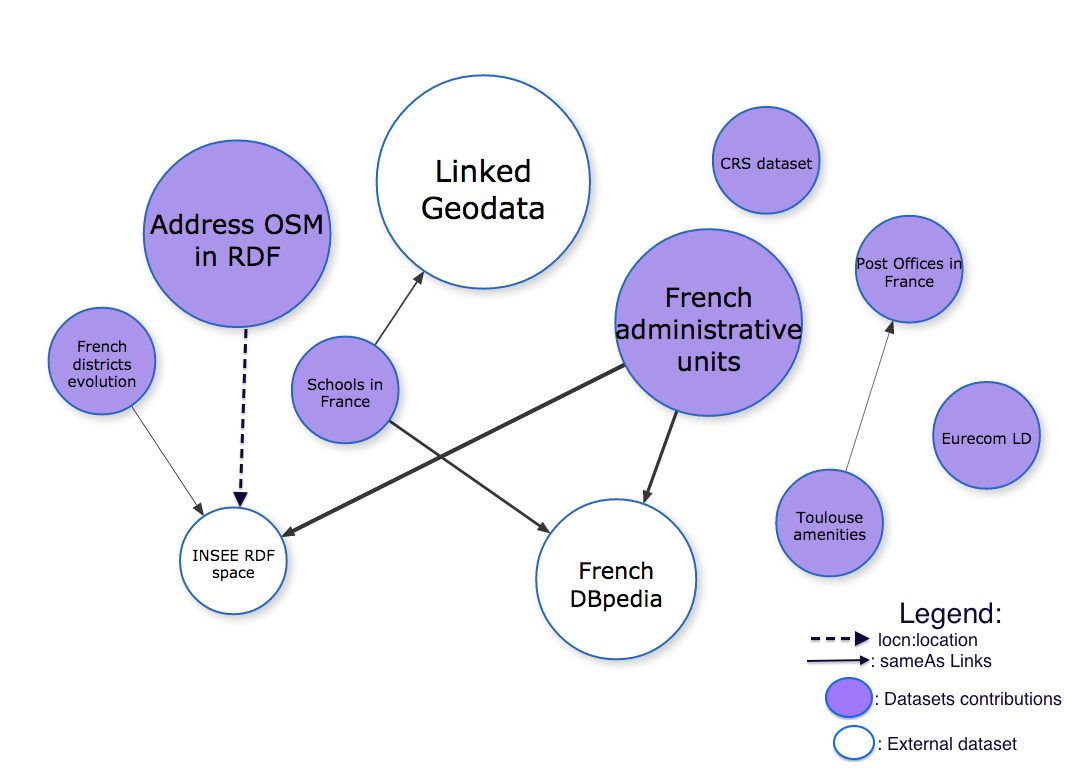
\includegraphics[width=\linewidth]{img/frenchCloud.png}
  
    \caption{French LOD Cloud based on the different datasets published in 4-5 stars. }
    \label{visuGraphModel}
  }
\end{figure}


\section{Opportunities and Challenges}\label{sec:challenges}

 The need for interoperable reference geographic data to share and combine georeferenced environmental spatial information is particularly acknowledged by the INSPIRE Directive. For geographic data producers, the benefit of publishing their data on the Web according to Linked Data  (LD) principles is twofold. On the one hand, their data are interoperable with other published datasets and they can be referenced by external resources and used as spatial reference data, which would not have been straightforward when published according to spatial data infrastructures (SDI) standards. On the other hand, the use of semantic Web technologies can help addressing interoperability issues which are not solved yet by geographic information standards. 
Moreover, there are different types of license policies to access data at IGN (e.g.: research purpose, commercial use, access on demand, etc.), with some of them not necessary ``open'' or free to access: (e.g. BD TOPO\circledR). Although there is a clear understanding of the benefits of publishing and interconnecting data on the web, ongoing investigations on how to combine licenses on datasets are under consideration at IGN. Two solutions are under investigation: (i) different license policies attached to datasets and (ii) the use of a security access mechanism on top of the datasets granting access based on a predetermined configuration on named graphs and resources. 
According to Linked data principles URIs should remain stable, even if administrative units change or disappear. This implies adapting the data vocabulary in order to handle data versioning and real world evolutions. This issue will be addressed in a future work, as we plan to release a spatio-temporal dataset describing the evolution of communes since the French Revolution. Another issue deals with the automation of the whole publication process, from traditional geographic data to fully interconnected RDF data.
The last issue deals with the use of multiple geometries for describing a geographic feature: geometries with different levels of detail, different CRS, different representation choices. This has been superficially addressed in our use case with the use of both polygons and points for representing respectively the surface and the centroid of departments, but should be further investigated for both query answering and map design purposes.


%The need for interoperable reference geographic data to share and combine georeferenced environmental spatial information is particularly acknowledged by the INSPIRE Directive. This is also true for any georeferenced thematic data, and especially in the context of the Web of data where location properties can be used with benefits for data linking purposes. Particularly, good quality reference geodatasets can be used as the spatial frame for anchoring and combining many thematic data. For geographic data producers, the benefit of publishing their data on the Web according to Linked Data  (LD) principles is twofold. On the one hand, their data are interoperable with other published datasets and they can be referenced by external resources and used as spatial reference data, which would not have been straightforward when published according to spatial data infrastructures (SDI) standards. On the other hand, the use of semantic Web technologies can help addressing interoperability issues which are not solved yet by geographic information standards. However, it may also has the drawback of publishing geographic data twice: following LD principles and according to SDI  standards. This raises the issue of proposing a mediation approach between data access solutions used by SDI and Linked Data.
%In this article, we have proposed a reference dataset on French administrative units. This dataset is updated annually by IGN France. This raises a first issue on how to deal with data updates and versioning. According to Linked data principles URIs should remain stable, even if administrative units change or disappear. This implies adapting the data vocabulary in order to handle data versioning and real world evolutions. This issue will be addressed in a future work, as we plan to release a spatio-temporal dataset describing the evolution of French communes since the French Revolution. Another issue deals with the automation of the whole publication process, from traditional geographic data to fully interconnected RDF data.
%Another issue deals with the use of multiple geometries for describing a geographic feature: geometries with different levels of detail, different CRS, different representation choices. This has been superficially addressed in our use case with the use of both polygons and points for representing respectively the surface and the centroid of departments, but should be further investigated for both query answering and map design purposes.

\subsection{Summary}
